% -*- root: ../main.tex -*-
\chapter{Sieci neuronowe}
\label{chap:nerual:nets}

Sieci neuronowe są jednym z najgorętszych tematów w świecie sztucznej inteligencji a może także poza nim. Mają one proste i eleganckie właściwości, które zostały zainspirowane myśleniem o podobnych systemach znajdujących się w mózgu. Pomimo tego, że ich genezą są modele mózgu, to teraz wiemy, że różnią się one od ich biologicznych odpowiedników na pewne ogromne sposoby. Na przykład prawdziwe neurony są aktywowane inaczej i mają prawdopodobnie inny mechanizm uczenia się. Ponieważ wiedza o mózgu jest ograniczona, nie możemy wiedzieć, czy tak jest na pewno. Czy te różnice są do pogodzenia, nie jest jeszcze pewnym. Wiemy, natomiast że sieci, które działają na naszych komputerach, mogą osiągać dosyć niesamowite wyniki. Jednak nie było tak zawsze. Jeszcze kilkadziesiąt lat temu wiele osób miało wątpliwości na temat tego, czy sieci neuronowe są w stanie dokonać niektórych rzeczy. To tak jakbyśmy przenieśli się w czasie do wynalazku silnika. Dla wielu osób w tym czasie nie było zapewne jasne, do czego można go użyć, a nawet jeśli zdawali sobie sprawę z niektórych zastosowań, to nie byli sobie w stanie wyobrazić innych. Podobnie na początku badania sztucznej inteligencji nie było wiadomo, co da się osiągnąć, a co jest, niemożliwe stosując te metody. Nie wiedziano nawet które problemy są łatwe a które ciężkie do rozwiązania. Niektórzy myśleli, że rozwiązanie problemów, które są ciężkie dla nas, takich jak różniczkowanie, będzie ciężkie również dla maszyn, a problemów łatwych dla nas, jak rozpoznawanie obiektów, będzie dla nich łatwe. Okazało się inaczej. Problem różniczkowania został rozwiązany dość szybko przez Jamesa Slagle’a, który napisał pierwszy program obliczający całki. Co ciekawe Slage był niewidomy, nie przeszkodziło mu to jednak w napisaniu programu całkującego w języku LISP. LISP był początkowo popularnym językiem programowania w kręgach ludzi zajmujących się sztuczną inteligencją. Był, można nawet powiedzieć, elitarnym językiem programowania. Dzięki swojej prostej i eleganckiej składni, która przypominała operowanie na listach, nowoczesnym rozwiązaniom oraz przede wszystkim traktowaniu każdego wyrażenia jak symbolu stał się on popularny w kręgach AI. LISP był też nietypowy, gdyż niektóre wyrażenia, które można naturalnie zapisać w innych językach, trzeba było napisać w sposób rekursywny, co stanowiło dodatkową trudność. LISP nie był językiem stworzonym dla sieci neuronowych. Jego wolne działanie w porównaniu do innych języków tamtego czasu, takich jak C, było przeszkodą dla algorytmów wymagających szybkości obliczeniowej. W tamtym czasie wielkich przełomów nie to było najważniejsze. Konceptualne przełomy dokonywały się jeden po drugim, a naukowcy dokonywali wielkich obietnic, ponieważ widzieli ogromny postęp w kilku formalnych dziedzinach. Problemy takie jak rozpoznawanie obiektów nadal pozostawały nierozwiązane. Kiedy okazało się niemożliwym, żeby rozwiązać inteligencję bez wcześniejszego poradzenia sobie z tymi ‘łatwiejszymi’ problemami przyszła tzw. zima AI (ang. AI winter), kiedy to fundusze na badania zostały ograniczone. Wszyscy byli zawiedzeni tym, co zostało osiągnięte, ponieważ spodziewano się jeszcze szybszych postępów, jednak ukryte problemy dawały znać. Dotknięta została również dziedzina badań nad sieciami neuronowymi, które w tamtym czasie nie dawały tak niezwykłych rezultatów. W konsekwencji tylko kilku najwytrwalszych naukowców kontynuowało badania nad sieciami neuronowymi. Byli to naukowcy z Kanady i jeden Francuz. W 2019 za badania prowadzone w czasie kiedy nikt nie wierzył w sieci neuronowe Hinton, Bengio i LeCun zostali nagrodzeni nagrodą Turinga. Istniał też inny realny problem poza wygórowanymi oczekiwaniami. Komputery lat 70 były dużo wolniejsze niż obecne. A jeśli jest jedna rzecz, która jest prawdziwa w stosunku do sieci neuronowych to to, że są ogromnie głodne zasobów. Było po prostu niemożliwym, żeby osiągnąć niektóre z niezwykłych rezultatów, które potrafimy dokonać obecnie na tamtych komputerach. Dzisiaj sieci neuronowe są używane we wszelakich rozwiązaniach, zaczynając od rozpoznawania liter, znaków, twarzy, przeprowadzania diagnozy medycznej, grania w gry komputerowe, szachy i Go, po wykonywanie za nas nużących czynności jak filtrowanie spamu czy wybieranie kolejnego filmu do odtworzenia albo piosenki do posłuchania.

\section{Perceptron}

Pomysł stojący za \textbf{perceptronem} jest prosty. Weźmy kilka danych wejściowych, połączmy je w pewien sposób i zwróćmy wartość numeryczną. Jeśli ta wartość jest większa niż zero, to klasyfikujemy dane wejściowe jako należące do klasy 0, w przeciwnym wypadku klasyfikujemy je jako klasę 1. Na ten pomysł wpadł Frank Rosenblatt w 1958 roku. Perceptron początkowo miał być nie programem a specjalną elektroniczno-elektro-mechaniczną maszyną zafundowaną przez amerykańskie wojsko. Rosenblatt ‘sprzedał’ wojskowym swój pomysł jako maszynę do rozpoznawania znaków na zdjęciach, choć oni wiązali z nim prawdopodobnie dużo większe nadzieje. Pomyślmy co moglibyśmy chcieć klasyfikować. Możemy np. chcieć sprawdzić, czy na zdjęciu jest kot, czy go tam nie ma albo sprawdzić, czy podana litera to ‘A’, czy nie. Jednak wojskowi pokładali zapewne największe nadzieje w rozpoznawaniu sprzętu wojskowego na zdjęciach. Jak miałoby to działać w perceptronie? Musimy mu najpierw przekazać nasze dane jako wejściowe, np. jeśli chcemy klasyfikować zdjęcia, powinniśmy mu dostarczyć listę wszystkich pikseli. Teraz musimy pomyśleć, jak chcemy połączyć wszystkie informacje, które otrzymuje perceptron. Na początku zmieniamy piksele w związane z nimi wartości numeryczne, a następnie mnożymy je przez jakąś pozytywną lub negatywną wagę. Kolejno musimy tylko dodać wszystkie wartości, które otrzymaliśmy i sprawdzić, czy ich suma jest większa, czy mniejsza od 0.

\begin{equation}
\begin{split}
f(x) = 1, \textrm{jeśli \space} w * x > 0
\\
\textrm{i \space} f(x) = 0 \textrm{\space w przeciwnym wypadku}
\end{split}
\end{equation}

\noindent W równaniu (3.1) $\boldsymbol{w}$ są wagami, przez które mnożymy dane wejściowe $\boldsymbol{x}$, następnie, jeśli suma jest większa niż 0, zwracamy jeden, inaczej zwracamy zero.\newline

Działanie perceptronu możemy zwizualizować jako oddzielanie płaszczyzny prostą linią. Z jednej strony takiej linii będą przykłady pozytywne, czyli te oznaczone jako 1, a z drugiej negatywne, czyli oznaczone jako 0. Ta linia będzie koniecznie przechodzić przez punkt (0, 0). Możesz to sprawdzić, wybierając jakieś wagi i wstawiając do równania $\boldsymbol{x}$ równe 0. Jeśli nie lubimy tej właściwości, a nie jest ona najbardziej pożądana ze względu na niemożliwość rozdzielenia pewnych zbiorów danych, to możemy dodać tzw. \textbf{współczynnik korygujący} (ang. bias) do każdej danej wejściowej. Więc:

\begin{equation}
\begin{split}
f(x) = 1, \textrm{jeśli \space} w * x + b > 0
\\
f(x) = 0 \textrm{ \space w przeciwnym wypadku}
\end{split}
\end{equation}

\noindent Jedyna zmiana następuje w pierwszej części równania (3.2), gdzie dodajemy wartości $\boldsymbol{b}$ do każdej danej wejściowej. I pamiętamy tu, że dodawanie następuje po mnożeniu.\newline

Co pozostało nam do zrobienia? Potrzebujemy jakoś określić wartość naszych wag, ale jest bardzo dużo możliwości, na które moglibyśmy to zrobić. Wagi mogą w teorii przyjmować wartość równą dowolnej liczbie rzeczywistej. Jednak aby poprawnie klasyfikowały nasze dane, konieczne jest, aby były odpowiednio dobrane. Tu z pomocą przychodzi rozdział 2.X. Możemy po prostu użyć algorytmu SGD na przykładach zdjęć z kotami. Żeby mogło to jednak zadziałać, potrzebna jest nam funkcja wartości, która będzie określać, jak dobrze zaklasyfikowaliśmy dany przykład. Jak dokładnie będzie wyglądać nasza funkcja wartości w tym przypadku? Funkcją wartości będzie dystans pomiędzy przykładem a \textbf{granicą decyzyjną}, tutaj naszą prostą $\boldsymbol{f(x) = 0}$. Dystans ten pomnożymy przez 1, jeśli zaklasyfikowaliśmy przykład poprawnie i -1, jeśli zrobiliśmy to błędnie. Zauważmy, że wartość funkcji wartości zależy od odległości przykładu od prostej. Sprawia to, że perceptron próbuje znaleźć najlepszą taką prostą, a także pomaga w uczeniu, poprzez pokazywanie jak daleko nasz przykład znajduje się od bycia źle zaklasyfikowanym. Pozostaje nam dodać ostatnią część. Moglibyśmy, co prawda, zrobić to, co opisaliśmy, ale byłoby koniecznym używać wszystkich przykładów do obliczania jednego kroku. Dzieje się tak, ponieważ nie mamy sposobu, aby zmienić wynik klasyfikacji za pomocą pojedynczego przykładu. Może nam się błędnie wydawać, że SGD rozwiązuje ten problem. Możemy przecież trenować po kolei na kolejnych przykładach, jednak musimy powiedzeć, że SGD nie wykorzystuje informacji, o tym, jak mocno dany piksel się ‘świeci’ do poprawy klasyfikacji. A zauważmy, że obecność danego piksela o określonym kolorze może świadczyć o obecności np. kota. SGD z funkcją wartości, którą opisaliśmy, spróbuje tylko znaleźć odpowiednie wagi, które prowadzą do najlepszej klasyfikacji, nie weźmie natomiast pod uwagę jakie elementy wejściowe przyczyniły się do osiągnięcia rezultatu. SGD zmienia wagi na korzystniejsze, patrząc się na przykłady tylko aby określić funkcję wartości, poza tym skupia się na zmienialnych parametrach czyli wagach. Chcemy aby nasze rozwiązanie nie zmieniało, w sposób ślepy wag, tylko brało pod uwagę to, w jaki sposób dane wejściowe mogą być skorelowane z klasyfikacją. Na pomoc przychodzi \textbf{reguła aktualizacji} perceptronu (ang. update rule). Jest ona jedną z najciekawszych jego części. Mówi nam ona, że:

\begin{equation}
w_i(t+1) = w_i(t) + (y - (w * x + b)) * x
\end{equation}

\noindent Gdzie $\boldsymbol{w_i(t)}$ są wagami w kroku $\boldsymbol{t}$, $\boldsymbol{y - (w * x + b)}$ jest różnicą między oczekiwanym rezultatem $\boldsymbol{y}$ a otrzymanym $\boldsymbol{w * x + b}$ a $\boldsymbol{x}$ jest wartością wejścia.\newline

Wszystkie elementy mają pewien sens, w świetle tego, o czym mówiliśmy. Zastosowaliśmy regułę rekurencyjną do aktualizacji wag. Do tego zmieniamy je o różnicę między oczekiwanym wyjściem a otrzymanym, używając pojęcia granicy decyzyjnej. Jedyne czego nie wiemy, to, skąd pojawiło się $\boldsymbol{x}$ na końcu równania. Możemy pomyśleć o sytuacjach, w których chcielibyśmy zwiększyć zmianę, którą aplikujemy do naszych wag. Co się dzieje, gdy zwiększamy ją gdy $\boldsymbol{x}$ jest duże i zmniejszamy gdy $\boldsymbol{x}$ jest małe? Zmiana będzie większa przy większych wartościach tej zmiennej, ale całkowita zmiana zależy też od różnicy pomiędzy spodziewanym a otrzymanym wynikiem, czyli od błędu przewidywania. A więc zmiana wag będzie wzmacniana, gdy jednocześnie błąd i wejście będą duże. Jeśli taka sytuacja ma miejsce, to znaczy, że $\boldsymbol{x}$ jest dobrym predyktorem tej różnicy, a więc waga odpowiadająca temu $\boldsymbol{x}$ powinna być zmieniona tak, aby była bardziej receptywna na to wejście. To właśnie osiąga reguła aktualizacyjna perceptronu. Jest to jeden z najważniejszych pomysłów dotyczących sieci neuronowych. Używając tej reguły, szukamy danych wejściowych, które dobrze przewidują błąd, a więc pomagają w otrzymaniu poprawnego wyniku.\newline

\clearpage
\begin{figure}[H]
\centering
\includepdf[pages=7]{mputo.pdf}
\caption{Perceptron}
\end{figure}
\clearpage

Czy wiedząc wszystko, co zostało zawarte w tym rozdziale, możemy iść i próbować klasyfikować koty? Prawdopodobnie nie. Mimo iż perceptron był zaprojektowany, by klasyfikować obrazy, jest on dość zły w tym zadaniu. Jedyne co robi perceptron, to tworzy oddzielającą przykłady płaszczyznę w $\boldsymbol{n}$ wymiarowej przestrzeni. Taka płaszczyzna oddzielająca jest zbyt mało skomplikowana, aby przedstawić większość różnic między przykładami np. kotów. Perceptron może być bardziej predysponowany, do powiedzmy, klasyfikacji domów na te zawierające basen i te go nie posiadające, używając do tego celu informacji na temat ceny, metrażu i dystansu do centrum miasta. Jeśli chodzi natomiast o bardziej złożone zastosowania, perceptron jest przestarzały, mając na uwadze obecne standardy. Może on mieć dosyć duże problemy z pewnymi specjalnie wybranymi, ale bardzo prostymi funkcjami takimi jak XOR (XOR jest funkcją która przyjmuje dwa argumenty, oba z nich są 0 albo 1, i zwraca 1, jeśli wejścia są różne i 0 w przeciwnym przypadku). W roku 1969 Marvin Minsky i Seymour Papert wydali słynną książkę o nazwie „Perceptrons”, która matematycznie udowadniała, że perceptron nie jest w stanie działać jak bramka XOR, co spowodowało w tamtym czasie spadek zainteresowania rozwiązaniami takimi jak perceptron, ponieważ wydawało się, że udowodniono, że sieci typu perceptron mają pewne nierozwiązywalne ograniczenia z nimi związane.



\section{Neurony}

O neuronach wiemy, wydaje się nam, intuicyjnie dużo, przecież towarzyszą nam każdego dnia. Jednak niestety żaden z nich nie raczył się nam przedstawić i objaśnić sposobu swojego działania. Pomogłoby to nam zapewne w podejmowaniu lepszych decyzji, jeśli wiedzielibyśmy, z jakich części składa się nasz mózg. Jednak przy braku takich kurtuazji pozostaje się nam zdać na nasze własne badania i dociekania na ten temat. W poszukiwaniu wyjaśnienia wewnętrznego działania mózgu ludzie stworzyli modele tego, co jest w środku. Jeden z najprostszy takich modeli był używany w perceptronie, który opisaliśmy poprzednio. Nie będziemy tu opisywać takich modeli prawdziwych neuronów ze względu na ortogonalność takiego przedsięwzięcia oraz brak wiedzy autora na ten temat. Co jednak zrobimy, to opiszemy modele używane w sztucznych sieciach neuronowych. Należy zaznaczyć, że te modele nie są identyczne i, według naszej wiedzy, różnią się od siebie w znaczący sposób. Przejdźmy więc do opisu wytworu naszej wyobraźni. Każdy sztuczny neuron posiada pewną liczbę $\boldsymbol{n}$  wejść, które zazwyczaj są liczbami rzeczywistymi. Celem takiego neuronu jest dokonanie pewnej transformacji tych danych wejściowych. Możemy niejako myśleć o działaniu pojedynczego neuronu jak o wyniku działania perceptronu, który klasyfikuje dane, które otrzymuje na pewne klasy. To był najpopularniejszy pogląd, na to, jak powinien działać neuron jeszcze kilkadziesiąt lat temu. Zazwyczaj klas, na które neuron miał klasyfikować wejście, było dwie. Jedna dla stanu aktywnego a druga dla stanu nieaktywnego. W ten sposób miała być oddana właściwość prawdziwych neuronów, które albo są, albo nie są aktywne w zależności od wejścia. W następnym podrozdziale zobaczymy jak połączenie neuronu z funkcją aktywacji, może dać podobny wynik. Jednak podstawową różnicą między perceptronem a neuronami jest to, że te drugie, jak możesz się domyślać, łączymy w większe sieci, składające się z wielu neuronów. Te większe sieci są podstawą potęgi neuronów. Tak jak to zostało udowodnione w komputerach, u mrówek czy u ludzi, nie siła pojedynczej jednostki decyduje o sile systemu, lecz raczej zbiorowe, skoordynowane działanie. Sieci neuronów wykorzystują efekt sieci i skali, aby się wzajemnie wzmacniać. Pomimo że działanie jednego neuronu jest proste i łatwe do opisania to działanie ich grup daje niespodziewane wyniki i jest ciężkie do ujęcia matematycznymi wyrażeniami w sposób przejrzysty dla człowieka. O tym też powiemy w następujących podrozdziałach. Wracając do działania neuronu, zazwyczaj każde wejście $\boldsymbol{x}$  zostaje na początku pomnożone przez wagę $\boldsymbol{w}$ , następnie dodajemy współczynnik korygujący $\boldsymbol{b}$, zupełnie jak w perceptronie, i sumujemy wszystkie rezultaty.\newline

\begin{equation}
u = \Sigma(x * w + b)
\end{equation}

Sumując wszystkie wartości $\boldsymbol{x * w + b}$ otrzymujemy pewien wynik $\boldsymbol{u}$. Moglibyśmy go uznać za wynik działania neuronu, jednak to znaczyłoby, że wynikiem mogłaby być dowolna liczba, co niekoniecznie jest wskazane. Pomyślmy, że taka liczba mogłaby być dowolnie mała lub duża, co sprawiałoby nie tylko problemy z przetworzeniem jej przez komputer, ale także mogłaby niszczyć wyniki działania wielu innych neuronów, jeśli zostałaby użyta wraz z ich wynikami do dalszych obliczeń. Z tego powodu chcemy, aby nasza wartość $\boldsymbol{u}$  została przetworzona przez tak zwaną \textbf{funkcję aktywacji}. Jest ona zazwyczaj nieliniowa, ponieważ nie chcemy, aby nasz neuron zachowywał się jak perceptron, to znaczy zawsze dzielił przestrzeń prostą linią. Jeśli użyjemy funkcji nieliniowej jako funkcji aktywacji, to podział przestrzeni będzie mógł być dużo bardziej złożony. Ta nieliniowość wprowadzona przez funkcję aktywacji sprawi, że podział będzie nieliniowy, a więc kilka połączonych ze sobą neuronów będzie mogło stworzyć dużo bardziej skomplikowany podział przestrzeni, niż taki, który moglibyśmy otrzymać bez funkcji aktywacji.\newline

\clearpage
\begin{figure}[H]
\centering
\includepdf[pages=8]{mputo.pdf}
\caption{Neuron}
\end{figure}
\clearpage


\section{Funkcje aktywacji}

\noindent Funkcja aktywacji $\boldsymbol{\phi}$ bierze jako wejście $\boldsymbol{u}$ i zwraca wyjście neuronu.

\begin{equation}
y = \phi(u)
\end{equation}

\noindent Wszystkie równania na neuron przedstawiają się następująco:

\begin{equation}
u = \Sigma(x * w + b)
\end{equation}
\begin{equation}
y = \phi(u)
\end{equation}

\noindent Pozostaje nam tylko dodać jakiej funkcji aktywacji należy używać. Funkcją, która była najbardziej popularna na początku wiedzy o sieciach neuronowych była \textbf{funkcja sigmoidalna} zdefiniowana jako:

\begin{equation}
S(x) = 1 / (1 - e^{-x})
\end{equation}

Ta funkcja ma kształt litery ‘S’. Zmienia się ona bardzo mało na końcach, a gradient jest największy blisko zera. Zwraca ona wartości pomiędzy 0 a 1, z tym że większość wartości leży blisko 0 lub 1 ze względu na kształt funkcji. Było to początkowo interesującą właściwością ze względu na podobieństwo do neuronów w mózgu, które albo są w stanie aktywacji, albo nie dają żadnego sygnału. Dodatkowym plusem jest nieliniowość tej funkcji. Pochodna funkcji sigmoidalnej jest prosta i jest to niewątpliwie silna strona ponad niektórymi konkurentami. Okazuje się jednak, że jest pewien duży problem z tą funkcją. Staje się ona w łatwy sposób nasycona, co znaczy, że jeśli $\boldsymbol{x}$ zmienia się znacząco to $\boldsymbol{y}$ zmienia się bardzo mało. Nasycenie w funkcji sigmoidalnej ma miejsce przy jej końcach. Kiedy takie nasycone funkcje zostają przez siebie pomnożone z wynikiem znajdującym się blisko zera, sprawia to, że wartość numeryczna staje się bardzo mała. Ponieważ komputery nie radzą sobie z arbitralną dokładnością, prowadzi to do niedokładności w obliczeniach gradientu podczas trenowania sieci neuronowej. Problemy z tego powodu nazywane są \textbf{znikającym gradientem} (ang. vanishing gradient). Może też wystąpić przeciwieństwo znikającego gradientu, kiedy duże wyniki funkcji są mnożone przez siebie, to może to prowadzić do eksplozji gradientu. Taka sytuacja jednak nie będzie mieć miejsca przy sigmoidalnej funkcji aktywacji, ponieważ jej wartość jest ograniczona do 1, natomiast przy innych funkcjach nieograniczonych z góry, jest to bardzo realne zagrożenie. Inną często używaną funkcją jest ReLU (ang. rectifier linear unit), ma ona skomplikowaną nazwę i bardzo prostą definicję:

\begin{equation}
R(x) = max(0, x)
\end{equation}

\clearpage
\begin{figure}[H]
\centering
\includepdf[pages=9]{mputo1.pdf}
\caption{Funkcje aktywacji}
\end{figure}
\clearpage

Jej wartość wynosi 0 dla negatywnych wartości $\boldsymbol{x}$ i jest równa dokładnie $\boldsymbol{x}$ dla wartości pozytywnych. W większości sytuacji powinno się używać ReLU zamiast funkcji sigmoidalnej, ponieważ daje ona lepsze empiryczne rezultaty. Ta funkcja ma dodatkową właściwość, będąc bardzo szybką do policzenia, co oszczędza cykle procesora. Możesz sobie myśleć: Poczekaj chwilę, czy ta funkcja nie jest przypadkiem liniowa? Odpowiedź brzmi: nie, nie jest liniowa ze względu na to, że jest ona liniowa tylko w pewnych jej częściach, które są połączone w punkcie (0, 0). Okazuje się, że to wystarcza, aby zapewnić bogate zachowanie dla całej sieci. Istnieją pewne wariacje na temat funkcji ReLU. Krótko opiszemy dwie z nich.\newline

\noindent Nieszczelne ReLU (ang. leaky ReLU) jest jednostką ReLU, która jest ‘nieszczelna’, to znaczy, że jeśli $\boldsymbol{x}$ jest mniejsze od zera, to nie zwraca ona 0 tylko zamiast tego $\boldsymbol{x}$ * 0,01, lub inną małą wartość zależną od $\boldsymbol{x}$.\newline

\noindent Parametryczne ReLU (ang. parametric ReLU) jest taki sam jak nieszczelne ReLU z tą małą różnicą, że nie mnożymy $\boldsymbol{x}$ przez 0,01 tylko przez $\boldsymbol{a}$ które jest znalezione w procesie uczenia. To kończy nasz krótki przegląd funkcji aktywacji.\newline

Funkcja sigmoidalna i ReLU stanowią dwie najważniejsze opcje, które mamy do wyboru tworząc model sieci neuronowej. Poza tym istnieją oczywiście inne możliwości, takie jak, chociażby tanges hiperboliczny. Faktem jest natomiast, że zazwyczaj dzielą kluczowe właściwości, silnie oraz słabe strony z jedną z dwóch opisanych tu funkcji. Z tego właśnie powodu ograniczyliśmy listę funkcji aktywacji do dwóch najważniejszych przykładów. Dodajmy, że perceptron posiadał swoją własną inną od tych tu opisanych funkcję aktywacji. Możesz teraz powrócić do rozdziału o perceptronie i zobaczyć czy ją rozpoznasz.


\section{Wszystko razem}

Teraz pokryliśmy wszystkie części budulcowe potrzebne do stworzenia sieci neuronowej. Możesz się siebie teraz pytać: Zaczekaj, czy nie mówiliśmy tylko o neuronach? Tak rozmawialiśmy tylko o neuronach, ale piękną rzeczą dotyczącą sieci neuronowych jest to, że potrzebują jako budulca tylko neuronów. Nie oznacza to, jednak że nie pozostało nam nic do zrobienia. Musimy się zastanowić nad jedną kluczową kwestią. Jak połączymy pewną liczbę neuronów w całość? Jest naprawdę wiele możliwości, na które moglibyśmy tego dokonać, bo każde wyjście neuronu możemy w teorii połączyć z wejściem dowolnego innego neuronu. Moglibyśmy nawet połączyć wyjście naszego neuronu z jego wejściem, tworząc swego rodzaju pętlę zwrotną. Mimo tej dowolności istnieją pewne rodzaje neuronów, które się zwyczajowo wyróżnia. Są to neurony, które mają trochę inne zastosowania. Nazywane są one \textbf{neuronami wejścia} i \textbf{wyjścia} (ang. input and output neurons). Widzimy, więc że te same części składowe w sieci neuronowej mogą pełnić różne funkcje. Neurony wejścia różnią się od innych tylko tym, że nie biorą informacji od innych neuronów, ale bezpośrednio z danych wejściowych. Neurony wyjścia za to, są często różnego, specjalnego typu, np. pozostawione bez funkcji aktywacji lub ich wynik jest tak zmieniony, aby zwracały dystrybucję prawdopodobieństwa. Pozwala to na swego rodzaju sformatowanie danych wyjściowych, aby nie były one ograniczone przez funkcję aktywacji. Pomyślmy teraz jak w sensowny sposób połączyć wiele neuronów w całość. Jeśli łączylibyśmy je losowo, to część połączeń byłaby odległych, to znaczy znacząco zmniejszałaby odległość na grafie pomiędzy danymi neuronami. Sprawiłoby to, że w sieci nie istniałabo pojęcie lokalności, ponieważ każdy neuron byłby połączony z odległymi, jak i bliskimi neuronami. Zazwyczaj jednak neurony układamy w tak zwane \textbf{warstwy} (ang. layers). To znaczy, że są zapakowane jeden obok drugiego w pewnej kolejności.

\begin{equation}
 warstwa = [n_1, n_2, n_3, …]
\end{equation}

W jednej sieci neuronowej możemy mieć wiele takich warstw. W tym momencie pojawia się oczywiste pytanie: Jak wiele ma być takich warstw i w jaki sposób mają być połączone? Niestety na pierwsze pytanie musimy odpowiedzieć tak jak poprzednio w takich sytuacjach. To zależy od sytuacji. Nie ma jednej najlepszej liczby warstw ani liczby neuronów w warstwie. To kolejna rzecz, którą możemy zmieniać, tworząc nasz model. Na pytanie na temat połączenia należałoby właściwie też odpowiedzieć, że to zależy od specyfiki architektury, np. istnieją specjalne rozwiązania przeznaczone do rozpoznawania obrazu. Nazywają się one CNN (ang. convolutional neural network) i wykorzystują konwolucje. O konwolucji możemy myśleć jak o pewnym okienku z określonymi wagami dla różnych pozycji w okienku. Takie okienko jest przesuwane przez obraz tak, że w różnych momentach zapisywane są wyniki z różnych części obrazu przetworzonej przez konwolucję. Te wyniki tworzą jakby nowy obraz, na których znowu używane są konwolucje. Wagi w konwolucjach podlegają normalnemu uczeniu podobnie jak w normalnych sieciach neuronowych. Takie konwolucje mają w teorii znajdywać pewne powtarzające się elementy na zdjęciu, takie jak krawędzie, rogi a w wyższych warstwach może np. rozpoznają części ciała takie jak oko, nos itd. Innym typem sieci neuronowej jest tak zwana \textbf{losowo połączona} sieć (ang. randomly wired network). Znaczy to, że neurony w pierwszej warstwie łączą się z losowymi neuronami w warstwie drugiej. Kolejne warstwy połączone są w ten sam sposób. Mimo iż moglibyśmy na tym zaprzestać, to nie wiedzielibyśmy czy neurony są połączone w najlepszy sposób. Najlepsze połączenie neuronów jest bardzo skomplikowanym problemem. Skąd w końcu mamy wiedzieć która informacja, z którego neuronu może się przydać dalej? Bardzo prostym rozwiązaniem jest wcale nie zastanawiać się nad tym problemem i neurony w kolejnej warstwie połączyć ze wszystkimi neuronami w warstwie poprzedzającej. W ten sposób każdy neuron w warstwie otrzymuje wszystkie informacje obecne w warstwie poprzedniej. Jest to nazywane \textbf{siecią w pełni połączoną} (ang. fully connected network). Jeszcze innym często wykorzystywanym typem sieci jest RNN (ang. recurrent neural network). Wspomnieliśmy już, że możemy w teorii podłączyć neurony do samych siebie. Tworzy to najprostszą sieć rekurencyjną. Sieci rekurencyjne są przydatne, gdy chcemy, żeby sieć była w stanie przechowywać jakieś dane. Zwykła sieć zwana jest feedforward network, co możemy luźno przetłumaczyć na „sieć przesyłu dalej”, jak sama nazwa wskazuje, przesyła tylko informacje do przodu, nie przechowując w pamięci żadnych informacji. Moglibyśmy zamknąć i ponownie otworzyć taką sieć pomiędzy klasyfikowaniem przykładów i otrzymać taką samą odpowiedź. Inaczej jest z RNN, zachowuje ona informacje pomiędzy przykładami, tak że informacja pokazana kiedyś może mieć wpływ na obecny wynik jej działania. Sieć RNN wymaga innego algorytmu propagacji wstecznej (o algorytmie propagacji wstecznej powiemy w następnym rozdziale), zwanego propagacją w czasie. Jeśli kiedykolwiek słyszałeś o sieci nueronowej, to mogło ci się wydawać, że musi to być coś bardzo skomplikowanego. Przecież proste rzeczy nie mogą być tak gorącym tematem debaty. Jednak jak sam widzisz budowa sieci neuronowej, jest bardzo prosta do matematycznego zdefiniowania i nie kryje w sobie wielkich tajemnic. To, co jest naprawdę skomplikowanym, to dopasowanie sieci do problemu, co wymaga szerokiej wiedzy i pewnego rodzaju myślenia przez analogię. Widzieliśmy, że do dobrania jest wiele parametrów, które teoretycznie mogą wpływać na wynik działania, choć zazwyczaj nie będą stanowiły żadnej różnicy. Pozostała nam teraz ostatnia, może najbardziej skomplikowana, część wiedzy, a mianowicie omówienie trenowania sieci neuronowych.

\clearpage
\begin{figure}[H]
\centering
\includepdf[pages=10]{mputo.pdf}
\caption{Sieć neuronowa}
\end{figure}
\clearpage

\section{Propagacja wsteczna}

Przed dyskusją na temat propagacji wstecznej powinniśmy omówić krótko, czym jest \textbf{propagacja} przez sieć neuronową (ang. forward pass). Przy każdej propagacji zaczynamy od podania sieci informacji wejściowych. Następnie informacje są przetwarzane przez pierwszą warstwę i informacje z niej są przesyłane do następnej warstwy do ponownego przetworzenia. Ten proces występuje dla wszystkich warstw, a dane przesuwają się od warstwy wejścia do warstwy wyjścia. Gdy ostatnia, wyjściowa warstwa zostaje osiągnięta, to wynik jest zwracany, a faza propagacji zostaje zakończona. Teraz stworzyliśmy pierwszą sieć neuronową, ale jest jeden problem, który występował również w perceptronie. Żeby nasza sieć robiła coś przydatnego, musimy znaleźć odpowiednie wagi, które dają poprawną odpowiedź. Przypomnijmy o jakich wagach mowa. Każdy neuron przetwarza informacje poprzez pomnożenie wejścia przez $\boldsymbol{w}$ wagi i dodanie $\boldsymbol{b}$ współczynnika korygującego a następne przetworzenie ich przez funkcję aktywacji. Każda waga oraz współczynniki korygujące dla każdego neuronu mogą być ustawione. O ustawianiu tych wag możemy myśleć nie jak o wybieraniu ich dla poszczególnych neuronów a zamiast tego, jak o ustawieniu wag dla całego modelu. Moglibyśmy po prostu stworzyć listę wag wszystkich neuronów i następnie spróbować ustawić je wszystkie naraz za pomocą algorytmu SGD. Przestrzeń, nad którą byśmy optymalizowali, miałaby ilość wymiarów równą ilości sumy wag wszystkich neuronów. Funkcją wartości mogłaby być odległość pomiędzy klasą, którą wybrała sieć a poprawną klasą. Jeśli sieć jest odpowiednio mała to, to podejście może odnieść sukces. Jeśli jednak naszą sieć tworzą tysiące neuronów, wydaje się dość mało prawdopodobnym, żeby wyszukiwanie w takiej wielowymiarowej przestrzeni mogło znaleźć odpowiednie wagi wszystkich neuronów. Pomyślmy o tym jak o strojeniu instrumentu. Łatwo byłoby nastroić instrument, oczywiście z odpowiednimi umiejętnościami, jeśli do zmiany jest tylko jedno ‘pokrętło’, jeśli jednak tych pokręteł jest kilkadziesiąt i na dodatek ustawiamy je wszystkie naraz, zamiast pojedynczo, to zadanie wydaje się prawie niemożliwe do wykonania. Przypomnijmy sobie, jak rozwiązany był podobny problem w perceptronie. Równanie (3.3) prezentujące regułę aktualizacji w perceptronie wygląda następująco:

\begin{equation}
w_i(t+1) = w_i(t) + (y - j(x)) * x
\end{equation}

\noindent Gdzie $\boldsymbol{w_i}$ były wagami, $\boldsymbol{x}$ było wejściem, a $\boldsymbol{j(x)}$ zdefiniujemy jako równe wyjściu $\boldsymbol{w * x + b}$ perceptronu.\newline

Możemy sobie wyobrazić użycie tej samej reguły do zmiany wag w sieci neuronowej. Znamy przecież $\boldsymbol{w}$, $\boldsymbol{x}$ oraz $\boldsymbol{j(x)}$ bo to po prostu wyjście neuronu. Skąd jednak weźmiemy spodziewaną wartość $\boldsymbol{y}$ dla każdego neuronu? Na pewno możemy ją dostać, dla neuronów, dla których zarówno spodziewany, jak i otrzymany wynik jest znany, czyli dla neuronów wyjścia. Problematyczne są jednak neurony znajdujące się w środkowych warstwach. Przesyłają one przecież informacje tylko do kolejnej warstwy, a przecież ta kolejna warstwa nie jest w stanie podać nam spodziewanego wyniku dla poprzedzających neuronów, bo spodziewana wartość jest znana dopiero dla ostatniej warstwy. Widzimy teraz, dlaczego sieci neuronowe z jedną warstwą są prostsze do stworzenia. Właśnie takie rozwiązania były początkowo wykorzystywane mimo swoich problemów, takich jak problem XOR. Byłoby jednak świetnie, gdyby istniała metoda przesyłania wartości oczekiwanej w głąb sieci, do wcześniejszych warstw neuronów. To pozwoliłoby nam na trenowanie wielowarstwowej sieci. I okazuje się, że taka metoda istnieje. Nazywa się \textbf{procedurą propagacji wstecznej} (ang. backpropagation). Używa ona zasady łańcuchowej, która jest formułą obliczania pochodnej funkcji złożonej. Zasada łańcuchowa mówi po prostu, że:

\begin{equation}
dx/dy = dx/dz * dz/dy
\end{equation}

\noindent Co może być ubrane w słowa w następujący sposób: pochodna (tu: zmiana) $\boldsymbol{x}$ względem $\boldsymbol{y}$ jest równa pochodnej $\boldsymbol{x}$ względem $\boldsymbol{z}$ pomnożonej przez pochodną $\boldsymbol{z}$ względem $\boldsymbol{y}$. Pozwala to na rozbicie jednej pochodnej na dwie inne.\newline


\noindent Nasza zasada aktualizacji dla metody gradientu (2.6) jest równa:

\begin{equation}
w_i(t+1) = w_i(t) - n * dE/dw
\end{equation}

\noindent Gdzie $\boldsymbol{w_i}$ są naszymi wagami, $\boldsymbol{n}$ jest stałą uczenia, a $\boldsymbol{dE/dw}$ jest pochodną błędu po wielkości wagi.\newline

Aby obliczyć nowe wagi dla naszej sieci koniecznie potrzebujemy znać \textbf{dE/dw}, lecz problemem jest to, że zazwyczaj nie możemy obliczyć tej pochodnej bezpośrednio dla neuronów znajdujących się na dowolnej głębokości w sieci. Zamiast tego użyjemy regułę łańcuchową. Możemy dzięki niej obliczyć pochodną funkcji cząstkowej, jeśli tylko znamy pochodną funkcji złożonej oraz równania wszystkich funkcji. Skupmy się na następującym przykładzie sieci neuronowej składającej się z trzech neuronów, dla którego chcemy obliczyć \textbf{dE/dw} dla neuronu \textbf{f}: 

\begin{equation}
y = h(f(w_1) + g(w_1))
\end{equation}

\noindent Załóżmy też, że znamy błąd określony równaniem:

\begin{equation}
e = E(h(z))
\end{equation}

\noindent Teraz aby obliczyć pochodną błędu dla \textbf{z} korzystamy z równania (3.12).
Zapiszmy pochodną:
 
\begin{equation}
dE/dw_1 = dE/dh * (dh/df * df/dw_1 + dh/dg * dg/dw_1)
\end{equation}

\noindent Co wynika po prostu z reguł różniczkowania. Użyliśmy reguły łańcuchowej oraz zasady obliczania pochodnej z sumy funkcji.\newline

\noindent Znając podane poniżej równania możemy obliczyć ich pochodne:
 
\begin{equation}
\begin{split}
e = E(h)
\\
y = h(f + g)
\\
f(w_1), g(w_1)
\end{split}
\end{equation}
 
To dawałoby nam możliwość podstawienia odpowiednich wyników do równania (3.16), obliczenie \textbf{dE/dw} i wstawienie rozwiązania do równania na aktualizację wag neuronów (3.13).\newline

Jedynym problemem jest to że nie potrafimy obliczyć tych pochodnych ogólnie, ponieważ zależą one również od konkretnego wejścia które otrzymają te funkcje. Tak więc podstawiając pochodne funkcji (3.17) do równania (3.16) otrzymujemy równanie zależne od wejścia \textbf{x} na pochodną błędu po wagach \textbf{dE/dw}:

\begin{equation}
dE(w_1, x)/dw_1 = dE/dh * (dh/df * df(w_1, x)/dw_1 + dh/dg * dg(w_1, x)/dw_1)
\end{equation} 


\noindent Następnie najłatwiejszym sposobem aby uzyskać wyniki numeryczne dla określonych wag \textbf{$w_1$} oraz wejścia \textbf{x} funkcji \textbf{f} jest obliczanie tych pochodnych razem z funkcjami, których wynik jest i tak konieczny do działania sieci. Dzięki temu kończąc propagację, będziemy znali wyniki wszystkich pochodnych cząstkowych \textbf{df, dg} koniecznych do obliczenia \textbf{dE/dw}. Jeśli obliczymy wcześniej równanie na \textbf{dE/dw} to będzie wystarczyło podstawić odpowiednie wartości, żeby uzyskać poszukiwaną zmianę dla naszych wag. To pozwoli nam zaktualizować wagi funkcji \textbf{f}.\newline

\noindent Przedstawimy teraz wyprowadzenie takiego równania dla w pełni połączonej sieci przesyłu do przodu (fully-connected feedforward net).\newline

\noindent Przypomnijmy sobie teraz równanie określające neuron (3.6), (3.7):

\begin{equation}
o = \phi(\Sigma(x * w + b))
\end{equation}

\noindent Gdzie \textbf{$\phi$} jest funkcją aktywacyjną, a $\boldsymbol{z = \Sigma(x * w)}$ cząstkowym wynikiem działania neuronu jak to wcześniej zdefiniowaliśmy.\newline

Żeby obliczyć pochodną błędu względem wag, będziemy musieli użyć reguły łańcuchowej dwukrotnie:

\begin{equation}
dE/dw = dE/do * do/dz * dz/dw
\end{equation}

\noindent Gdzie $\boldsymbol{dE/do}$ jest pochodną błedu względem wyniku działania neuronu, $\boldsymbol{do/dz}$ jest pochodną wyniku działania neuronu względem jego wyniku sprzed uzycia funkcji aktywacji, a $\boldsymbol{dz/dw}$ jest pochodną wartości neuronu przed funkcją aktywacji względem wagi $\boldsymbol{w}$.\newline

\noindent Jedyne co zrobiliśmy, to przepisaliśmy pochodną błędu, bo łatwiej będzie nam znaleźć pochodne z prawej strony równania. Teraz weźmy pod uwagę $\boldsymbol{do/dz}$. Jest, to, jak napisaliśmy pochodna wyniku działania neuronu względem wyniku sprzed użycia funkcji aktywacji. Biorąc więc pod uwagę równanie (3.7), możemy zapisać pochodną funkcji aktywacji:

\begin{equation}
do/dz = d \phi(z)/dz
\end{equation}

Pochodna $\boldsymbol{do/dz}$ jest równa pochodnej funkcji aktywacji. Przypomnijmy sobie, jakie mieliśmy funkcje aktywacji. Pochodne funkcji sigmoidalnej (3.8) i ReLU (3.9) to odpowiednio:

\begin{equation}
dS(x)/dx = S(x)(1 - S(x))
\end{equation}

\begin{equation}
\begin{split}
R = 1, \text{jeśli } x > 0,
\\
R = 0, \text{jeśli } x < 0,
\\
\text{i } R = 1 \text{ albo } 0\text{, jeśli } x = 0
\end{split}
\end{equation}

\noindent Tutaj, ponieważ ReLU jest nieróżniczkowalne w punkcie $\boldsymbol{x}$ = 0, musimy wybrać wartość pochodnej dla tego punktu sami.\newline

\noindent Znamy $\boldsymbol{do/dz}$, przejdźmy więc do pochodnej $\boldsymbol{dz/dw}$ z równania (3.20). Jest ona równa pochodnej wnętrza funkcji aktywacji (3.19):

\begin{equation}
dz/dw_i = d \Sigma(x * w) / d w_i = x_i
\end{equation}

\noindent Gdzie $\boldsymbol{dz/dw_i}$ jest pochodną wnętrza funkcji aktywacji względem wag, $\boldsymbol{x_i}$ jest ‘i’ wejściem neuronu. Dla neuronu w środowej warstwie $\boldsymbol{x_i}$ jest równe $\boldsymbol{o_j}$ wyjściu ‘j’ poprzedniej warstwy. Więc w generalnym przypadku: $\boldsymbol{x_i}$ = $\boldsymbol{o_j}$, a tylko dla pierwszej warstwy $\boldsymbol{x_i}$ = \textbf{i-te wejście}.\newline\newline

\noindent Teraz podstawiając równania (3.20), (3.21), (3.24) do równania (3.13) otrzymujemy:

\begin{equation}
w_i(t+1) = w_i(t) - n * dE/do * d \phi(z)/dz * o_j
\end{equation}

\noindent To będzie nasze równanie aktualizacji wag. Znamy w nim wszystkie wartości oprócz $\boldsymbol{dE/do}$. Tylko w ostatniej warstwie $\boldsymbol{dE/do}$ jest znane. Dla innych warstw musimy obliczyć tę wartość. Ponieważ nasza sieć jest w pełni połączona, to błąd dla poprzedniej warstwy zależy od wszystkich pochodnych w kolejnej warstwie:

\begin{equation}
dE/do = d(z_i, z_j, z_k, ...) / do
\end{equation}

\noindent Gdzie $\boldsymbol{z_N}$ oznacza błąd dla $\boldsymbol{N}$ neuronu w kolejnej warstwie. Przypomnijmy, że: $\boldsymbol{dE/do}$ jest pochodną błedu względem wyniku działania neuronu. Bład ten będzie jednak pochodził od wszystkich neuronów w kolejnej warstwie, ponieważ nasz neuron jest połączony z wszystkimi neuronami w kolejnej warstwie.

\clearpage
\begin{figure}[H]
\centering
\includepdf[pages=11]{mputo.pdf}
\caption{Pochodne w propagacji wstecznej}
\end{figure}
\clearpage

\noindent Teraz biorąc pochodną zupełną równania (3.32), otrzymujemy:
\begin{equation}
dE/do = \Sigma(dE/do_1 * do_1/dz_1 * dz_1/ do)
\end{equation}
\begin{equation}
dE/do = \Sigma(dE/do_1 * d \phi(z_1)/dz_1 * w_ij)
\end{equation}

\noindent Jedynka na końcu oznacza, że chodzi o następną warstwę.
$\boldsymbol{dz_1/do}$ = $\boldsymbol{w_{ij}}$ ponieważ $\boldsymbol{dz_1/do}$ = $\boldsymbol{d \Sigma(w * o) / do}$ = $\boldsymbol{w_{ij}}$. A $\boldsymbol{d \phi(z_1)/dz_1}$ jest pochodną kolejnej warstwy funkcji aktywacji\newline

$\boldsymbol{dE/do_1}$ jest pochodną błędu względem wejścia następnej warstwy funkcji aktywacji, ale jeśli następna warstwa jest warstwą wyjścia, to jak powiedzieliśmy wcześniej $\boldsymbol{dE/do_1}$ jest znane, ponieważ oznacza pochodną błędu względem wyjścia ostatniej wartwy. Teraz, jeśli policzymy $\boldsymbol{dE/do_1}$ dla przedostatniej warstwy i użyjemy go w poprzedniej warstwie, tak jak użyliśmy $\boldsymbol{dE/do_1}$ dla obliczenia $\boldsymbol{dE/do}$ to otrzymamy formułę rekursywną na obliczanie pochodnej błędu względem wyjścia kolejnych poprzednich wyjść neuronów. W algorytmie propagacji wstecznej przesuwamy się od końca sieci do jej początku, obliczając $\boldsymbol{dE/do}$ dzięki formule rekursywnej, używając faktu, że wartość $\boldsymbol{dE/do_1}$ jest znana dla neuronów wyjścia, ponieważ w tym przypadku $\boldsymbol{o}$ = $\boldsymbol{y}$.

\begin{equation}
dE/do_1 = dE(y) / dy
\end{equation}

\noindent Dla ostatniej warstwy możemy w łatwy sposób policzyć pochodną błędu względem $\boldsymbol{y}$ używając technik różniczkowania. Jednak jeśli znamy $\boldsymbol{dE/do_1}$ dla warstwy wyjścia to możemy, używając równania (3.28) policzyć $\boldsymbol{dE/do_1}$ dla warstwy przed warstwą wyjścia. Możemy tę czynność powtarzać dla kolejno poprzednich warstw, aż dojdziemy do wejścia. Korzystając z następujących równań, możemy policzyć, w jaki sposób powinniśmy zmienić wagi w sieci:

\begin{equation}
w_i(t+1) = w_i(t) - n * dE/do * d \phi(z)/dz * o_j
\end{equation}
\begin{equation}
dE/do = \Sigma(dE/do_1 * d \phi(z_1)/dz_1 * w_{ij})
\end{equation}

\noindent Warto powiedzieć, że równanie (3.30) i (3.31) mogą być wykonywane niezależnie. Np. w bibliotece PyTorch równanie (3.31) dla każdej warstwy jest wykonywane, kiedy wykonywana jest propagacja wsteczna. Równanie (3.30) jest natomiast wykonywane, dopiero kiedy sami podamy taką komendę. Oznacza to, że gradient jest obliczany niezależnie od ustawiania wag.\newpage


\section{Zaawansowane tematy w zagadnienu}

W poprzednich podrozdziałach przypatrywaliśmy się bliżej podstawowemu\break wprowadzeniu do sieci neuronowych. Nauczyliśmy się, jak możemy je zbudować, używać propagując przez nie dane i trenować używając algorytmu propagacji wstecznej. Jeśli nie zrozumiałeś poprzedniego rozdziału, proponujemy tutaj pewną alternatywną, rzadziej używaną metodę trenowania sieci neuronowych. Możemy myśleć o wagach w naszym modelu jak o genomie organizmu. Każda waga koduje w tym modelu określone zachowania. Bardziej sprawny organizm daje większą wartość funkcji wartości. W celu znalezienia lepszych organizmów użyjemy metod programowania genetycznego, krzyżując najlepsze organizmy z nadzieją, że efektem będą jeszcze sprawniejsze jednostki. Następnie przetestujemy je na naszym problemie. Wybierzemy kilka najbardziej sprawnych i znów skrzyżujemy jednostki dające najlepszy wynik. Jest to podejście symulujące ewolucję wykorzystane w celu poprawy naszych wag. Ten sposób trenowania sieci, choć zazwyczaj bardziej wymagający obliczeniowo, jeśli damy mu wystarczająco dużo czasu da nam równowartościowe rezultaty do metody propagacji wstecznej.\newline

Mówiliśmy, że celem sieci neuronowej jest minimalizacja funkcji wartości, ale nie powiedzieliśmy jeszcze wprost jakie typy takiej funkcji istnieją. W uczeniu maszynowym wyróżnia się dwa główne typy zadania. Jest to \textbf{klasyfikacja} i \textbf{predykcja}. Klasyfikacja polega na przypisaniu przykładu do odpowiedniej klasy, np. jak w przykładzie z kotami do klasy kotów lub braku kotów na zdjęciu. W ten sposób możemy klasyfikować przeróżne rzeczy: chociażby wykrywać twarze lub stwierdzić czy narośle rakowe jest niebezpieczne. Inną możliwością klasyfikacji jest klasyfikacja do wielu klas. W ten sposób możemy klasyfikować np. litery, gatunki zwierząt czy ceny. Aby dokonać klasyfikacji w sieci neuronowej, należy zwrócić liczbę od 0 do 1 w przypadku klasyfikacji dwuklasowej. W przypadku klasyfikacji wieloklasowej należy zwrócić \textbf{n} elementową dystrybucję prawdopodobieństwa [$x_1, x_2, … x_n$], gdzie każdy element oznacza prawdopodobieństwo, że dany przykład należy do danej klasy. Lista ta powinna się sumować do 1. Wyróżniliśmy też inny sposób działania sieci neuronowych i nazwaliśmy go predykcją. Predykcja polega na przewidywaniu jakiejś wartości. Możemy przewidywać np. temperaturę, wyniki wyborów czy wielkość PKB. To wszystko są wartości numeryczne w pewnym przedziale, więc nasza sieć będzie zwracać liczbę naturalną. W tym wypadku wyjściem może być, odpowiednio zeskalowane, normalne wyjście pojedynczego lub kilku neuronów.\newline

\clearpage
\begin{figure}[H]
\centering
\includepdf[pages=12]{mputo.pdf}
\caption{Normalizacja danych}
\end{figure}
\clearpage

Przed wprowadzeniem danych do sieci neuronowej chcemy je często przetworzyć w jakiś sposób. Działa tutaj zasada mówiąca, że lepsza reprezentacja prowadzi do lepszych rezultatów. Ta maksyma odnosi się zresztą, również do ludzi. Wolelibyśmy, powiedzmy grać w szachy, używając do tego planszy niż mówić na głos nasze ruchy, mimo iż oba rozwiązania opisują tę samą grę. Podobny fenomen możemy obserwować w sieciach neuronowych. One też lepiej radzą sobie z pewnymi rodzajami informacji niż innymi mniej przystosowanymi do bycia wejściem. Dlatego my chcąc osiągnąć jak najlepsze rezultaty, przetwarzamy dane w pewien sposób, licząc na to, że poprawi to wynik działania sieci. Przetwarzanie danych przed użyciem ich w sieci neuronowej często składa się z \textbf{normalizacji}. Normalizacja to proces skalowania danych wejściowych.
Popatrzmy na prosty przykład:\newline

\noindent Zmierzyliśmy temperaturę w przeciągu siedmiu kolejnych dni i otrzymaliśmy w wyniku zbiór danych $\boldsymbol{D}$.\newline

\begin{equation}
D = [1000000, 1000310, 1000070, 999960, 999760, 1000050, 1000540]
\end{equation}

\noindent Widzimy, że zmierzone temperatury są bardzo duże. Trenowanie na tym zbiorze będzie ciężkie, ponieważ relatywne różnice między punktami danych są niewielkie, dużo lepiej byłoby odjąć od każdego takiego punktu 1000000, otrzymując nowy zbiór $\boldsymbol{D_s}$.\newline

\begin{equation}
D_s = [0, 310, 70, -40, -240, 50, 540]
\end{equation}

\noindent Teraz nawet dla nas dane stały się bardziej przejrzyste. Ten zbiór leży w bardziej naturalnym przedziale i zazwyczaj trenowanie na nim będzie łatwiejsze. System nie będzie się musiał uczyć ignorować dużych wielkości i zwracać uwagę tylko na liczby na niższych miejscach. Zauważmy też, że niektóre dane zmieniły się z pozytywnych wartości na ujemne. Nie będzie to miało jednak efektu na wynik działania sieci, ponieważ informacja o relatywnych różnicach między przykładami została zachowana.\newline

Ponieważ pozyskiwanie dużych zbiorów danych jest często kosztowne, ludzie używają mniejszych zbiorów w pętli, przetwarzając przykłady po kilka razy w trakcie treningu. Ta praktyka, mimo iż może zwiększyć nasze możliwości trenowania sieci, prowadzi też często do pewnych niepożądanych konsekwencji. Znany efekt z tym związany jest nazywany \textbf{nadmiernym dopasowaniem} (ang. overfitting), co znaczy, że sieć osiąga dobre wyniki na zbiorze używanym do ćwiczenia, ale słabe w prawdziwym użytkowaniu albo na zbiorze testowym.\newline

\noindent \textbf{Zbiór testowy} jest zbiorem, na którym nie trenujemy, po to, aby uzyskać bezstronną ocenę naszego modelu.\newline

Zobaczmy, w jaki sposób może się objawiać nadmierne dopasowanie. Powiedzmy, że mamy pewien zbiór punktów, który może być opisany prostą linią albo trochę lepiej za pomocą skomplikowanego wielomianu. Jeśli do nauczenia tego dopasowania zostało użytych niewiele przykładów, mielibyśmy tendencje, żeby powiedzieć, że wielomian jest prawdopodobnie nadmiernym dopasowaniem, ponieważ nie jest prawdopodobne, by dobrze opisywał przykłady, których nie użyliśmy do jego stworzenia. Jeśli jednak przykładów było więcej, a dane nadal wskazują, że wielomian jest dobrym dopasowaniem do danych, to uzyskaliśmy potwierdzenie i teraz może bardziej sensownym wyborem jest wielomian, niż linia prosta. Nadmierne dopasowanie może się objawiać w sieci neuronowej jako zapamiętywanie przykładów. Mimo iż klasyczna sieć neuronowa nie ma pamięci, to jednak może przechowywać pewne informacje w swoich wagach. Czasami zdarza się, że taka sieć, zamiast np. uczyć się, z jakich części składają się koty, żeby przewidywać czy na zdjęciu jest kot, zapamiętuje konkretne informacje związane z podanym zdjęciem. Później wystarczy, że sieć ‘przypomni’ sobie, że widziała dane zdjęcie, aby zaklasyfikować je jako zdjęcie zawierające lub niezawierające kota. Dzieje się tak zazwyczaj, gdy sieć, której używamy, jest duża a przykładów, których używamy do trenowania, jest niewiele. W celu zapobiegania zjawisku otrzymywania lepszych rezultatów, ale tylko na papierze, zostały wymyślone metody \textbf{regularyzacji}. Jednymi z nich są tak zwane regularyzacja L1 i L2, które dodają do funkcji wartości pewną karę zależną od wielkości wag w naszej sieci. Funkcja wartości zmienia się następująco:

\begin{equation}
min(V_n) = min(V) + |w|
\end{equation}
\begin{equation}
min(V_n) = min(V) + |w|^2
\end{equation}

\noindent Gdzie równanie (3.34) opisuje regularyzację L1, a (3.35) regularyzację L2. Różnicą jak widać, jest potęga, do której podnosimy wagi, jednak w obu przypadkach wartość wag jest wartością bezwzględną.\newline

Taka zmiana w funkcji wartości spowoduje, że nasza sieć nie będzie trenować, tylko aby zwiększać zadaną wartość, co jest dla nas negatywnym skutkiem, ale za to sprawi, że wagi będą pod presją, aby pozostawać mniejsze. Jest to niewątpliwie pozytywny skutek, biorąc pod uwagę eksplodujący gradient. Także ilość połączeń będzie kontrolowana, ze względu na to, że niepotrzebne połączenia będą zmniejszane, bo poprawi to funkcję wartości. Ta mniejsza liczba połączeń, tak jak w naszym przykładzie z dopasowywaniem linii, sprawi, że wytrenowany model będzie prostszy, co zazwyczaj skutkuje lepszą generalizacją.\newline

Idea, która stoi za obecnym dużym sukcesem sieci neuronowych, jest następująca rekomendacja. Jeśli chcemy zwiększyć osiągnięcia sieci neuronowej na danym problemie, to chcemy zwiększyć jej rozmiar, jeśli nie zauważamy poprawy w funkcji wartości podczas treningu. Natomiast jeśli widzimy poprawę podczas treningu, ale nie jest ona widoczna na zbiorze testowym, to powinniśmy zwiększyć wielkość zbioru, na którym trenujemy. Ten wzrost liczby przykładów w zbiorze treningowym jest naturalnym sposobem regularyzacji. Widzimy, że samym zwiększaniem wielkości sieci i ilości danych jesteśmy w stanie poprawić wynik osiągany na naszym problemie. Jest to rzadko spotykana właściwość w świecie informatyki, gdzie zazwyczaj każde zachowanie trzeba zakodować w sposób bezpośredni, gdyż komputery cechują się wielką karnością i ogromnym brakiem wyobraźni. Taki jest klasyczny obraz sytuacji. Jednak sieci neuronowe udowadniają coś przeciwnego. Odpowiednio zaprogramowany komputer może być kreatywny, nie poruszać się utartymi schematami, a nawet uczyć się na własną rękę. Jest to naprawdę wielki przełom, który pozwala nam mieć nadzieję, że będziemy w stanie w przyszłości wykorzystywać do pożytecznych celów moc obliczeniową, która do tej pory rośnie w sposób wykładniczy. Wzrost wykładniczy oznacza że wzrost danej wielkości przyspiesza bardzo szybko. Jest to jeden z niewielu zasobów, które zachowują się w ten sposób. Połączenie tej ogromnej mocy z technikami przetwarzania danych może dawać nam nadzieję na przełom, który może nastąpić w najbliższej przyszłości.

